\section{Containers structure and use}
\begin{frame}
Container technology is not very old \newline
\vspace{0.5cm}
The most famous: 
\includegraphics[width=0.2\textwidth]{images/docker_logo2.png} \newline
\vspace{0.5cm}
Solomon Hykes was inspirated by container port in the world travel \newline
\vspace{0.5cm}
\centering{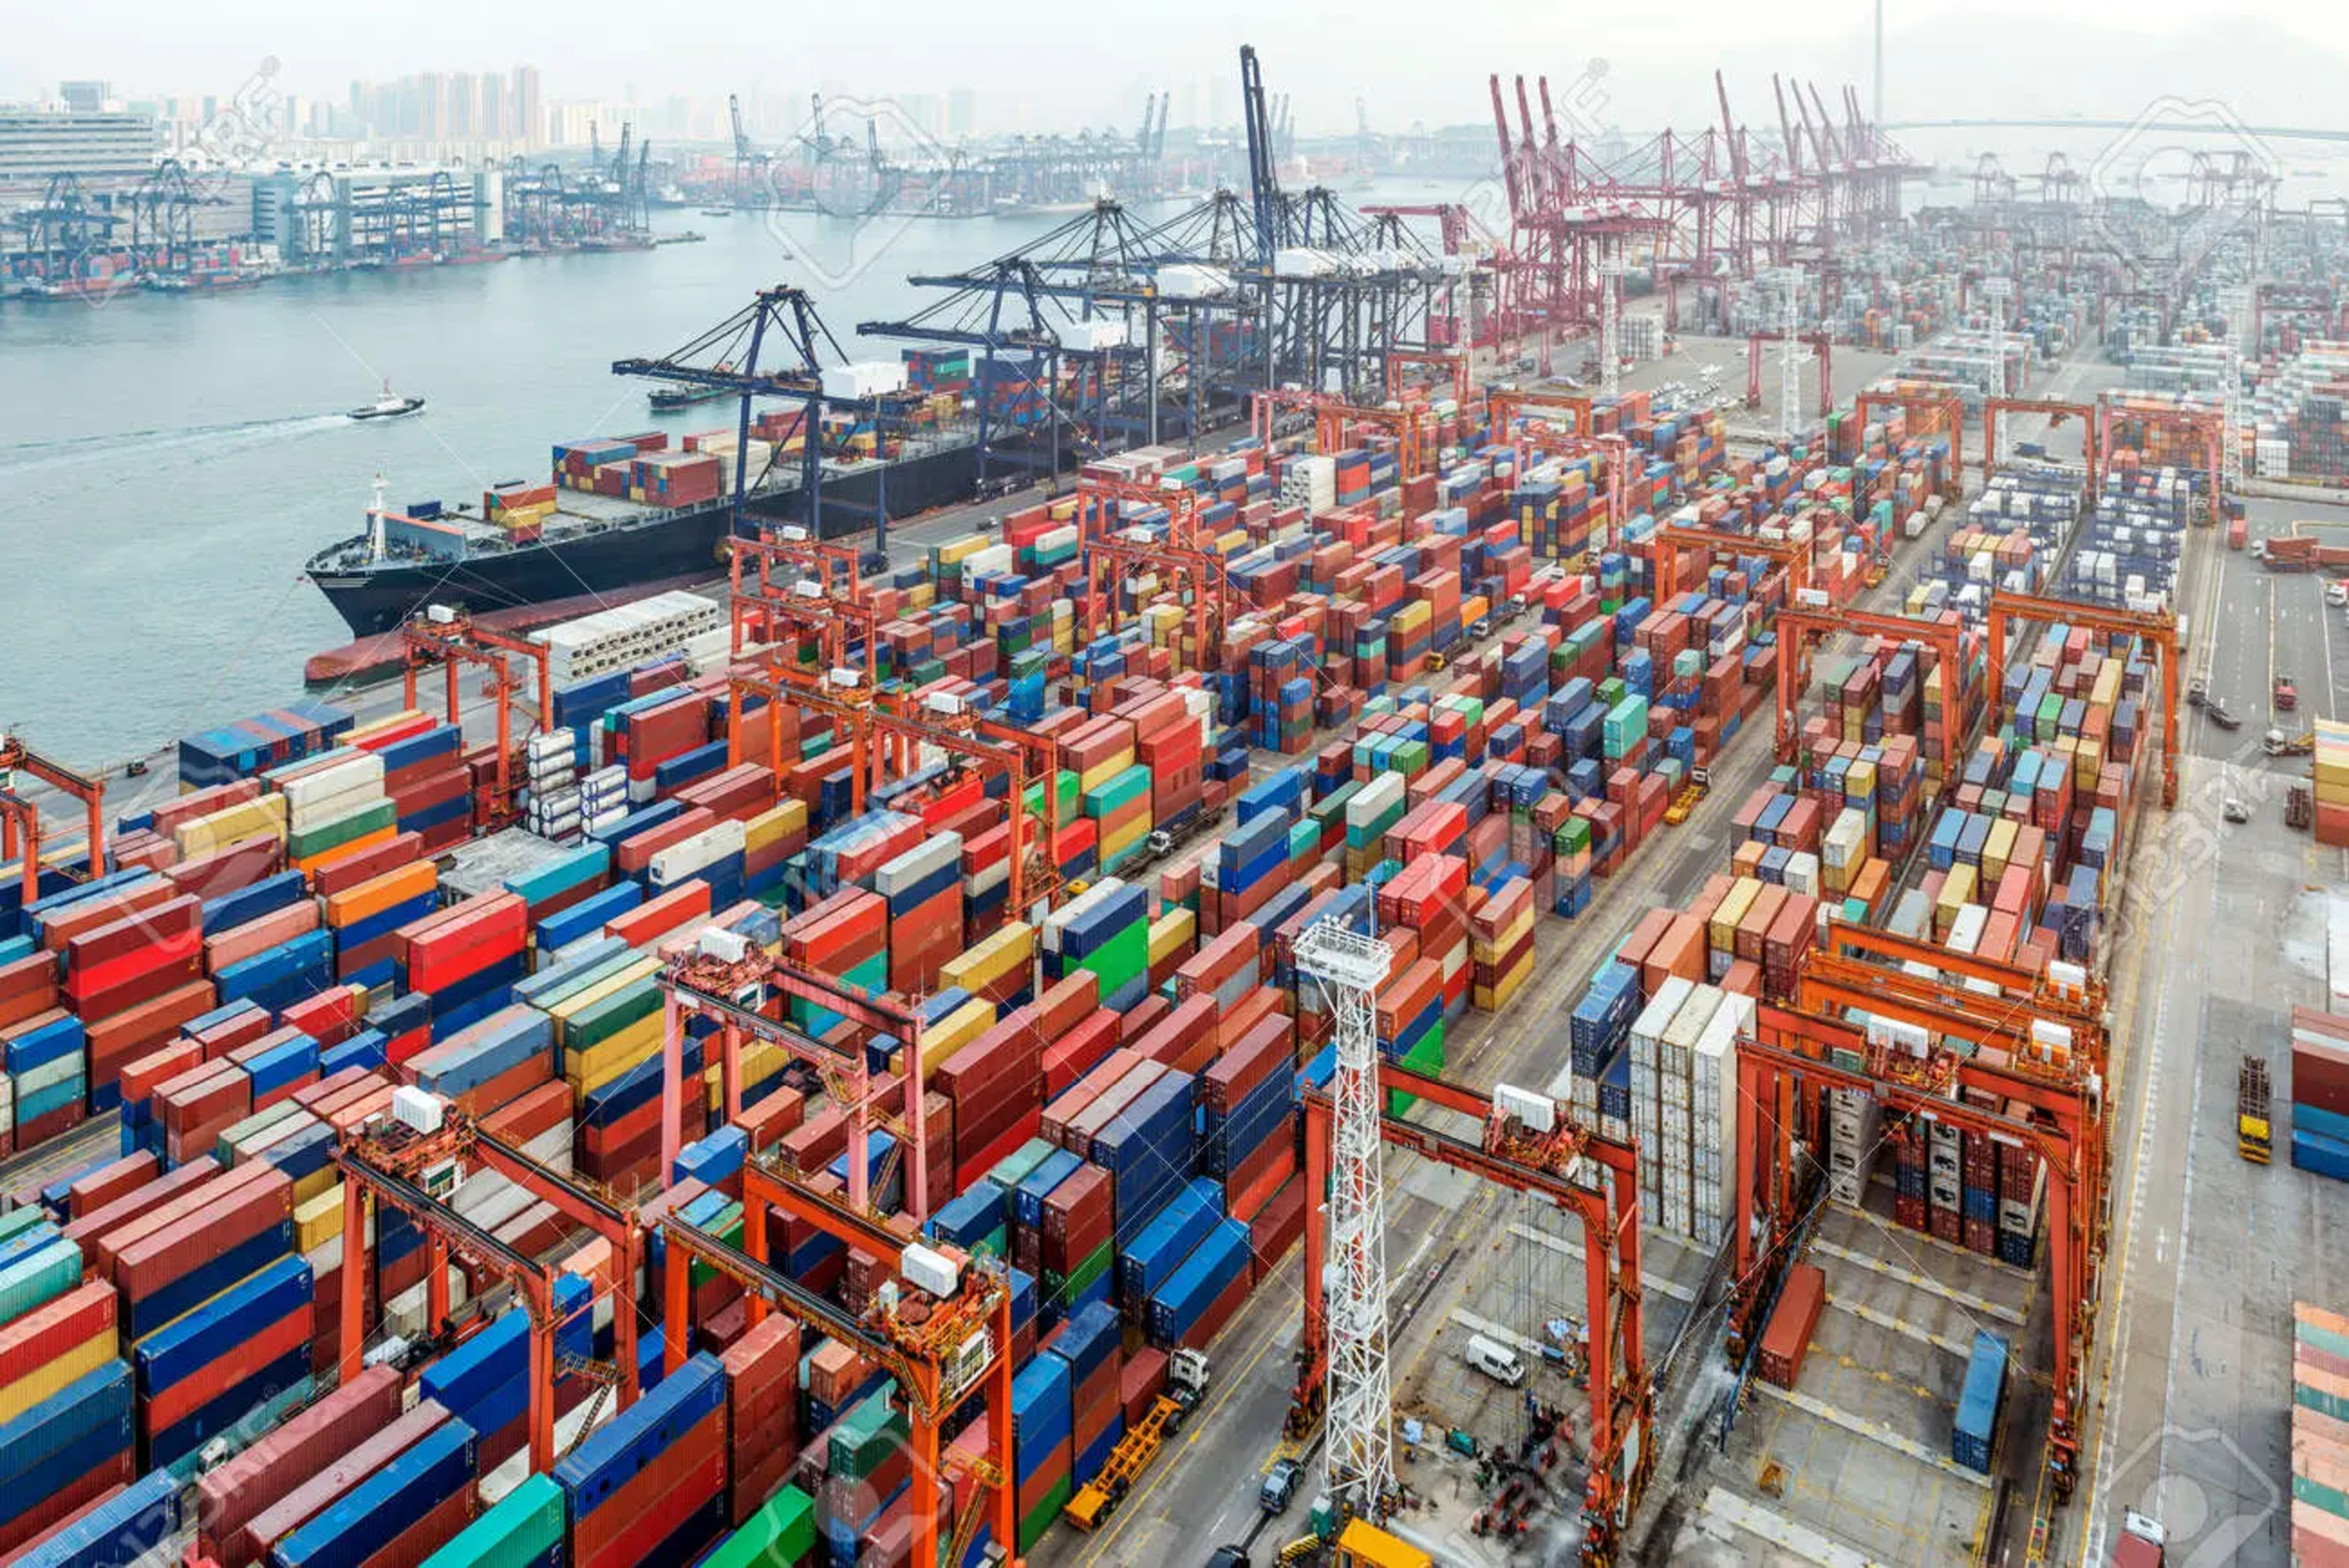
\includegraphics[width=0.4\textwidth]{images/container_port.pdf}} \newline
Docker is an open source project, a community and a private company 
\end{frame}

\begin{frame}
\begin{itemize}
\item Born in 2010
\item First public release in 2013
\item V 1.0 in 2014
\item Open source and free
\item Packaged to Ubuntu in 2014 (V14.04)
\end{itemize}
\end{frame}

\subsection{Docker}{Term definitions}
\begin{frame}
\begin{columns}
\column{.48\textwidth}
\begin{itemize}[<1->]
\item Docker image --> "snapshot" immutable file
	\begin{itemize}
	\item Set of libraries, functions
	\item Static state
	\item Online Store or share
	\item Automatically build
	\end{itemize}
\end{itemize}
\column{.48\textwidth}
\begin{itemize}[<2->]
\item Docker container --> instance of an image
	\begin{itemize}
	\item Result of the image activation
	\item Can be modified
	\item Can be tunred into an image
	\item 1 image --> multiple containers 
	\end{itemize}
\end{itemize} 
\end{columns}
\end{frame}

\begin{frame}{Docker architecture}
client-server architecture \\
\centering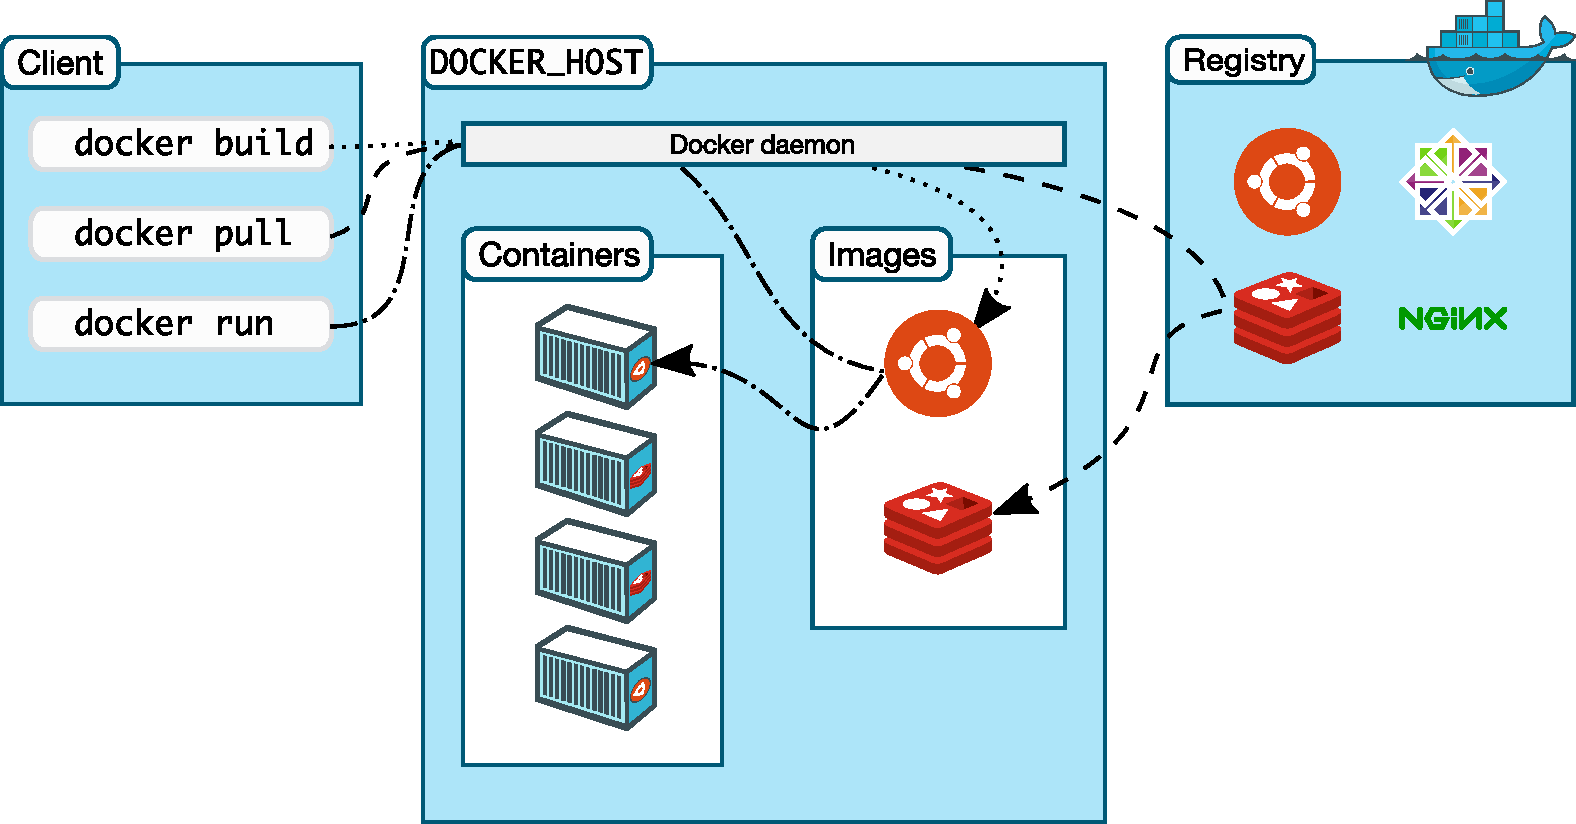
\includegraphics[width=0.8\textwidth]{images/docker_arch_3.pdf}
\end{frame}

\begin{frame}[fragile]{Docker client}
\begin{enumerate}
\item<1-> Client to interact with Docker
\item<2-> Client talk to the daemons (Docker background programs)
\begin{block}{Client}
\begin{verbatim}
$ docker build [path][url] 
  docker build https://github.com/docker/rootfs.git#container:docker
$ docker pull [image_name]
  docker pull biocontainers/samtools
$ docker run [image_name]
  docker run biocontainers/samtools
\end{verbatim}
\end{block}
\end{enumerate}

\begin{center}
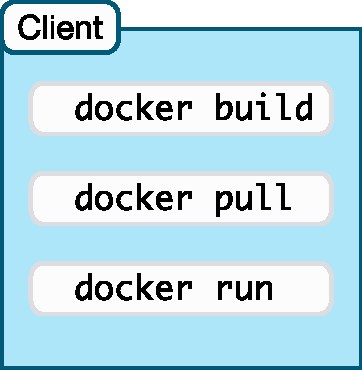
\includegraphics[width=0.15\textwidth]{images/docker_arch_1.pdf}
\end{center}
\end{frame}

\begin{frame}[<+->]{Docker daemon}
\begin{enumerate}
\item Listen client requests
\item Manage Dockers images, containers...
\end{enumerate}
\centering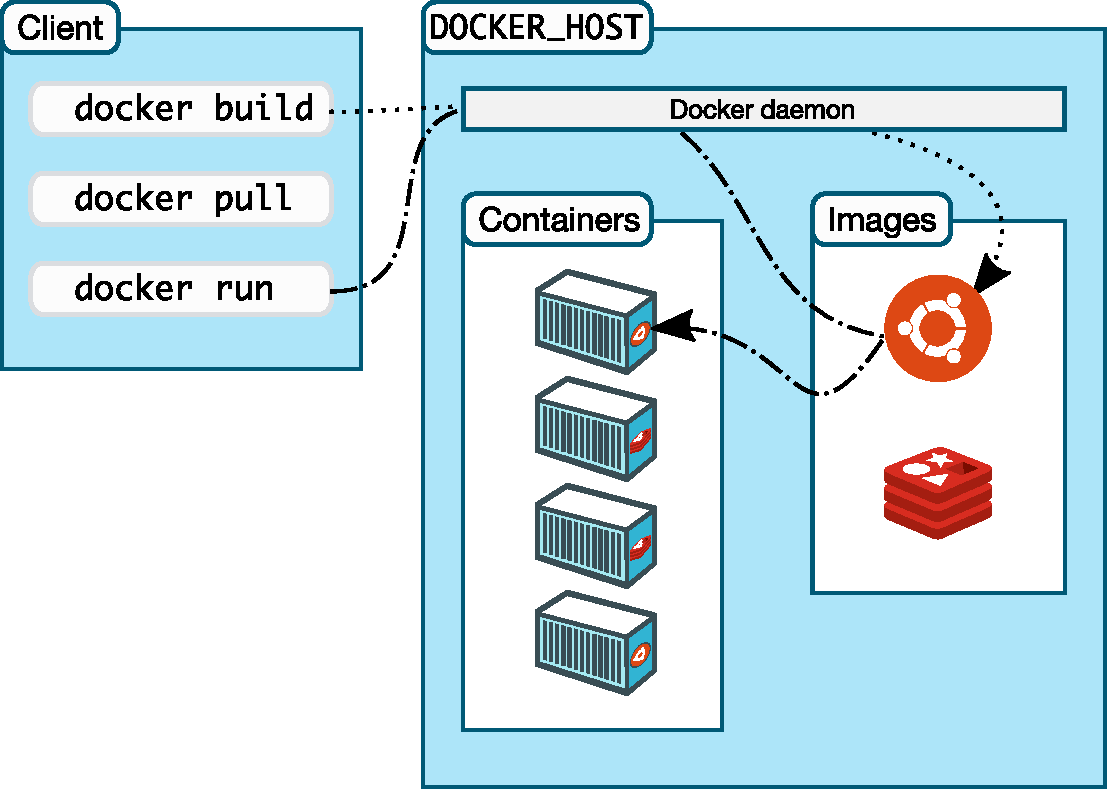
\includegraphics[width=0.6\textwidth]{images/docker_arch_2.pdf}
\end{frame}

\begin{frame}[<+->]{Docker registries}
\begin{enumerate}
\item Store Docker images
\item Docker hub is a public registry
\item You can run your own registry
\end{enumerate}
\onslide<2->{\centering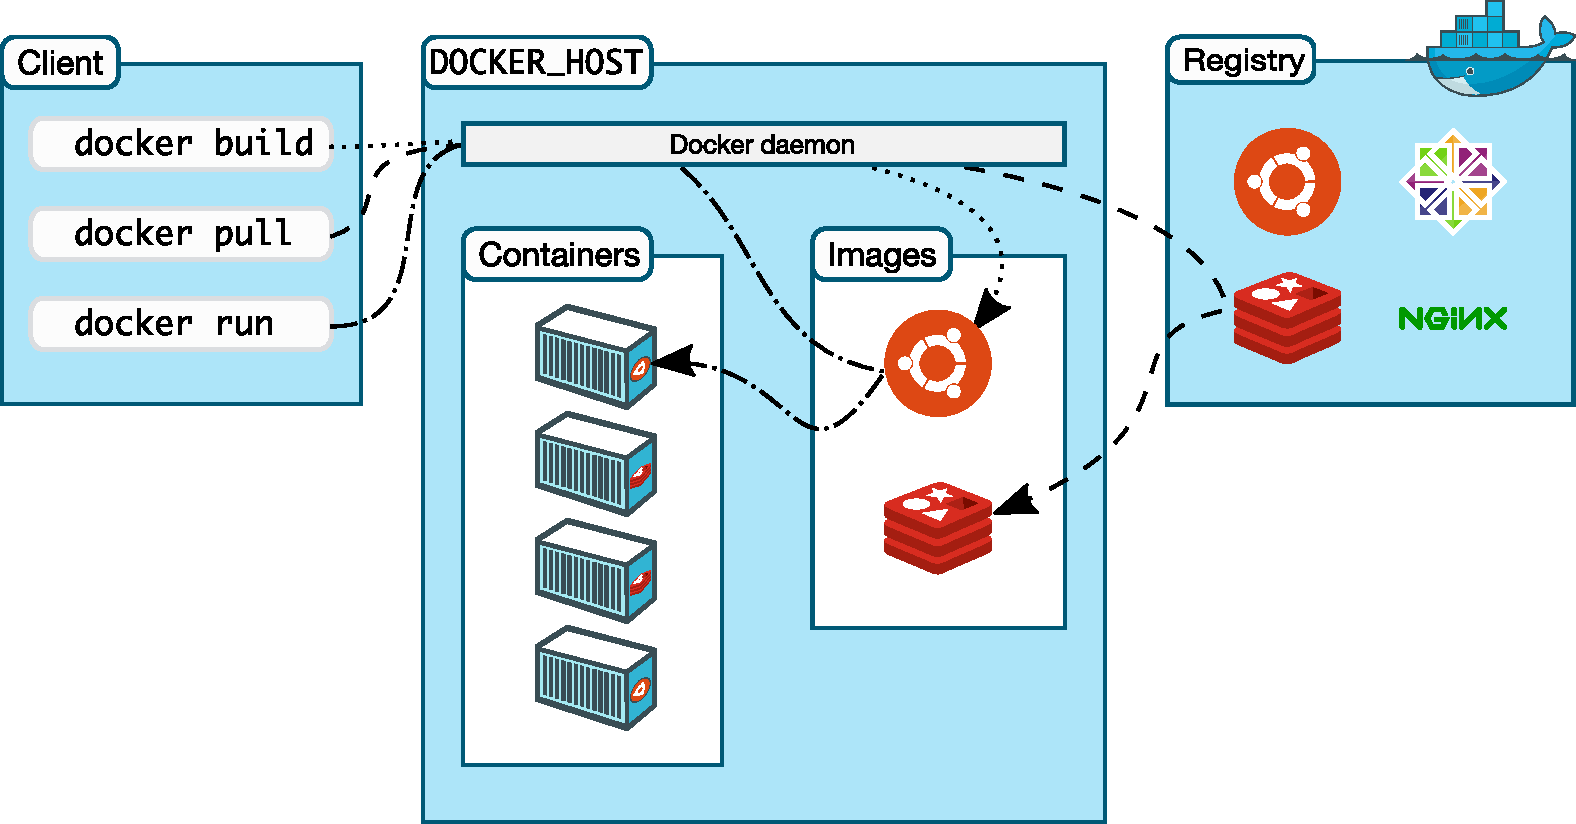
\includegraphics[width=0.75\textwidth]{images/docker_arch_3.pdf}}
\begin{textblock*}{10cm}(1cm,2cm)
\only<1>{\centering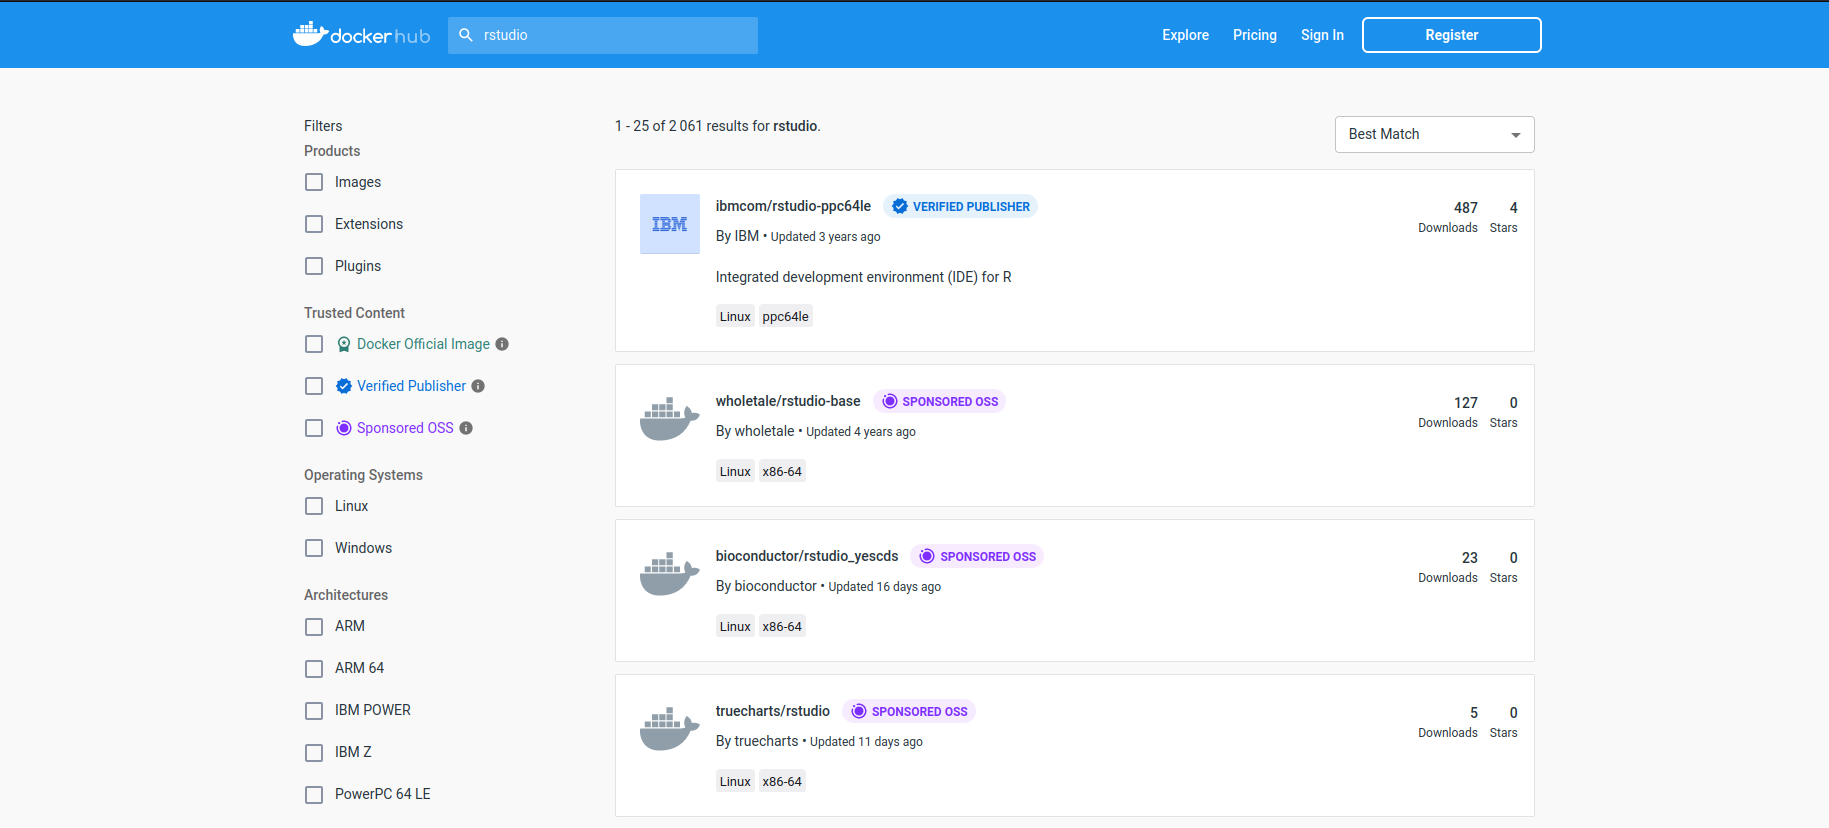
\includegraphics[width=1.4\textwidth]{images/docker_hub.png}}
\end{textblock*}
\end{frame}

\begin{frame}[fragile]{Image layers}
Focus on image building
\begin{itemize}[<+->]
\item Layers building
\item Several layers to one image
\end{itemize}
\end{frame}

\begin{frame}[fragile]{Image layers}
Focus on image building
\begin{itemize}
\item Layers building
\item Several layers to one image
\item Some layers shared by images when pulling
\item Lightheight the download and use of image on you computer
\end{itemize}
\begin{verbatim}
$ docker pull debian
Using default tag: latest
latest: Pulling from library/debian
fdd5d7827f33: Pull complete
a3ed95caeb02: Pull complete
Digest: sha256:e7d38b3517548a1c71e41bffe9c8ae6d6d29546ce46bf62159837aad072c90aa
Status: Downloaded newer image for debian:latest
\end{verbatim}
\end{frame}

\begin{frame}
\centering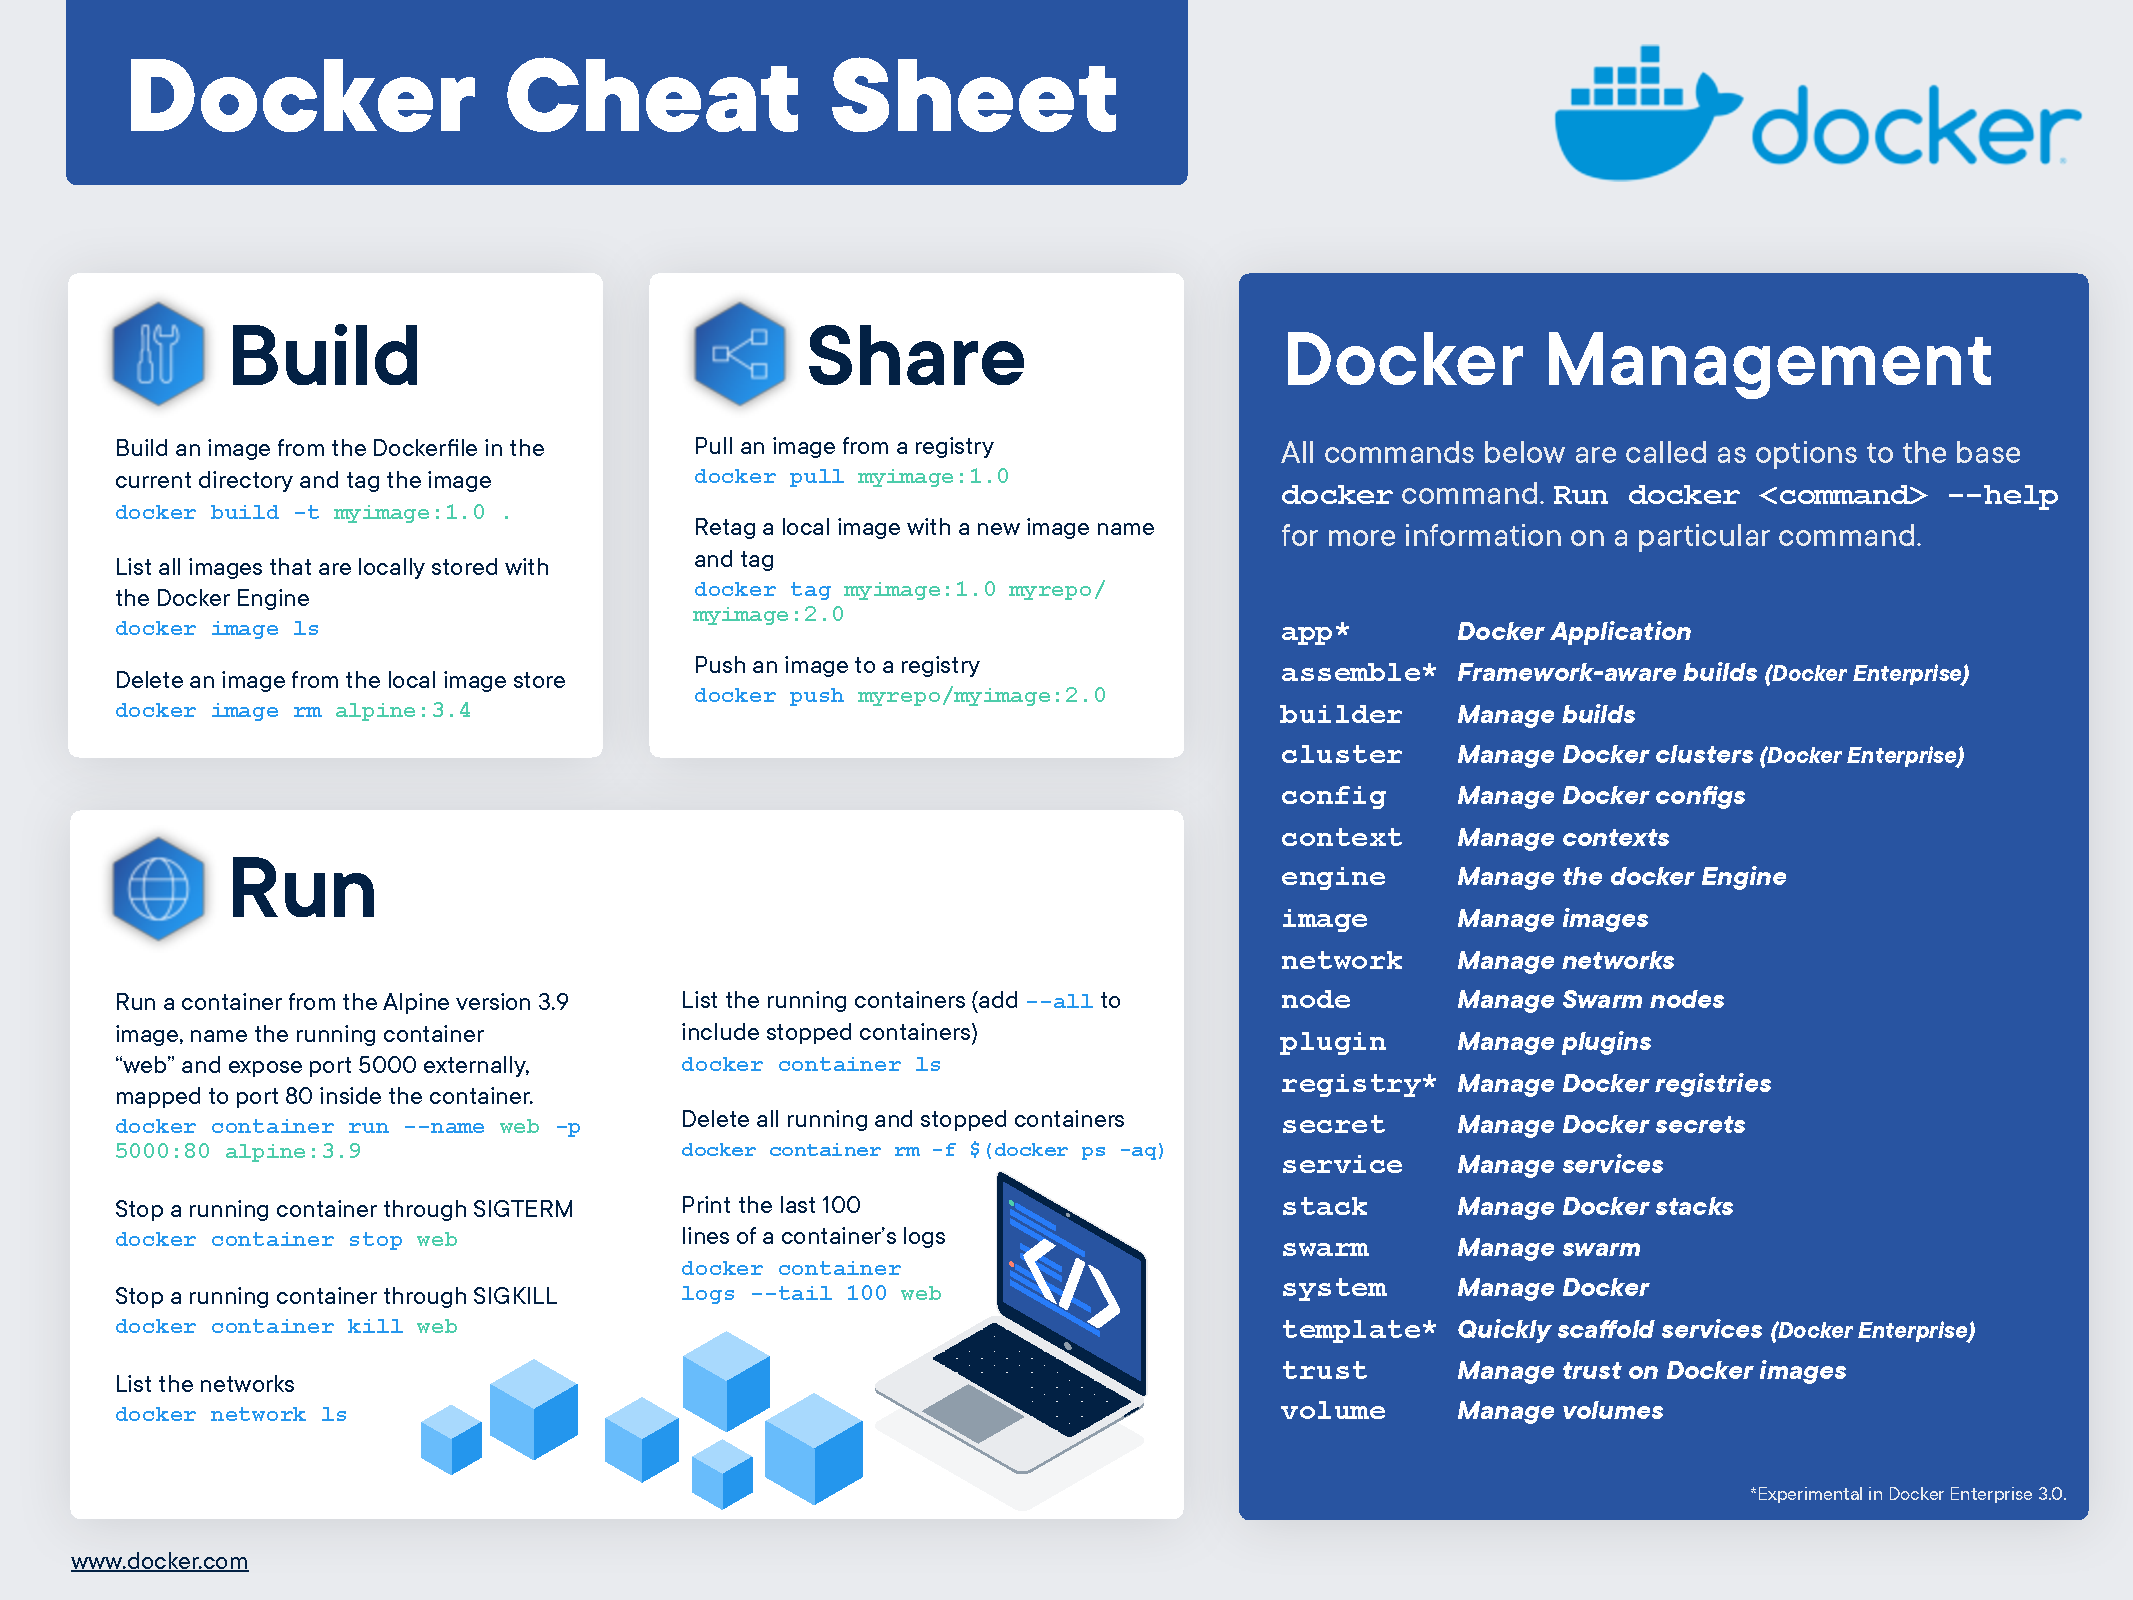
\includegraphics[width=0.9\textwidth]{images/docker-cheat-sheet.pdf}
\end{frame}

\begin{frame}
\centering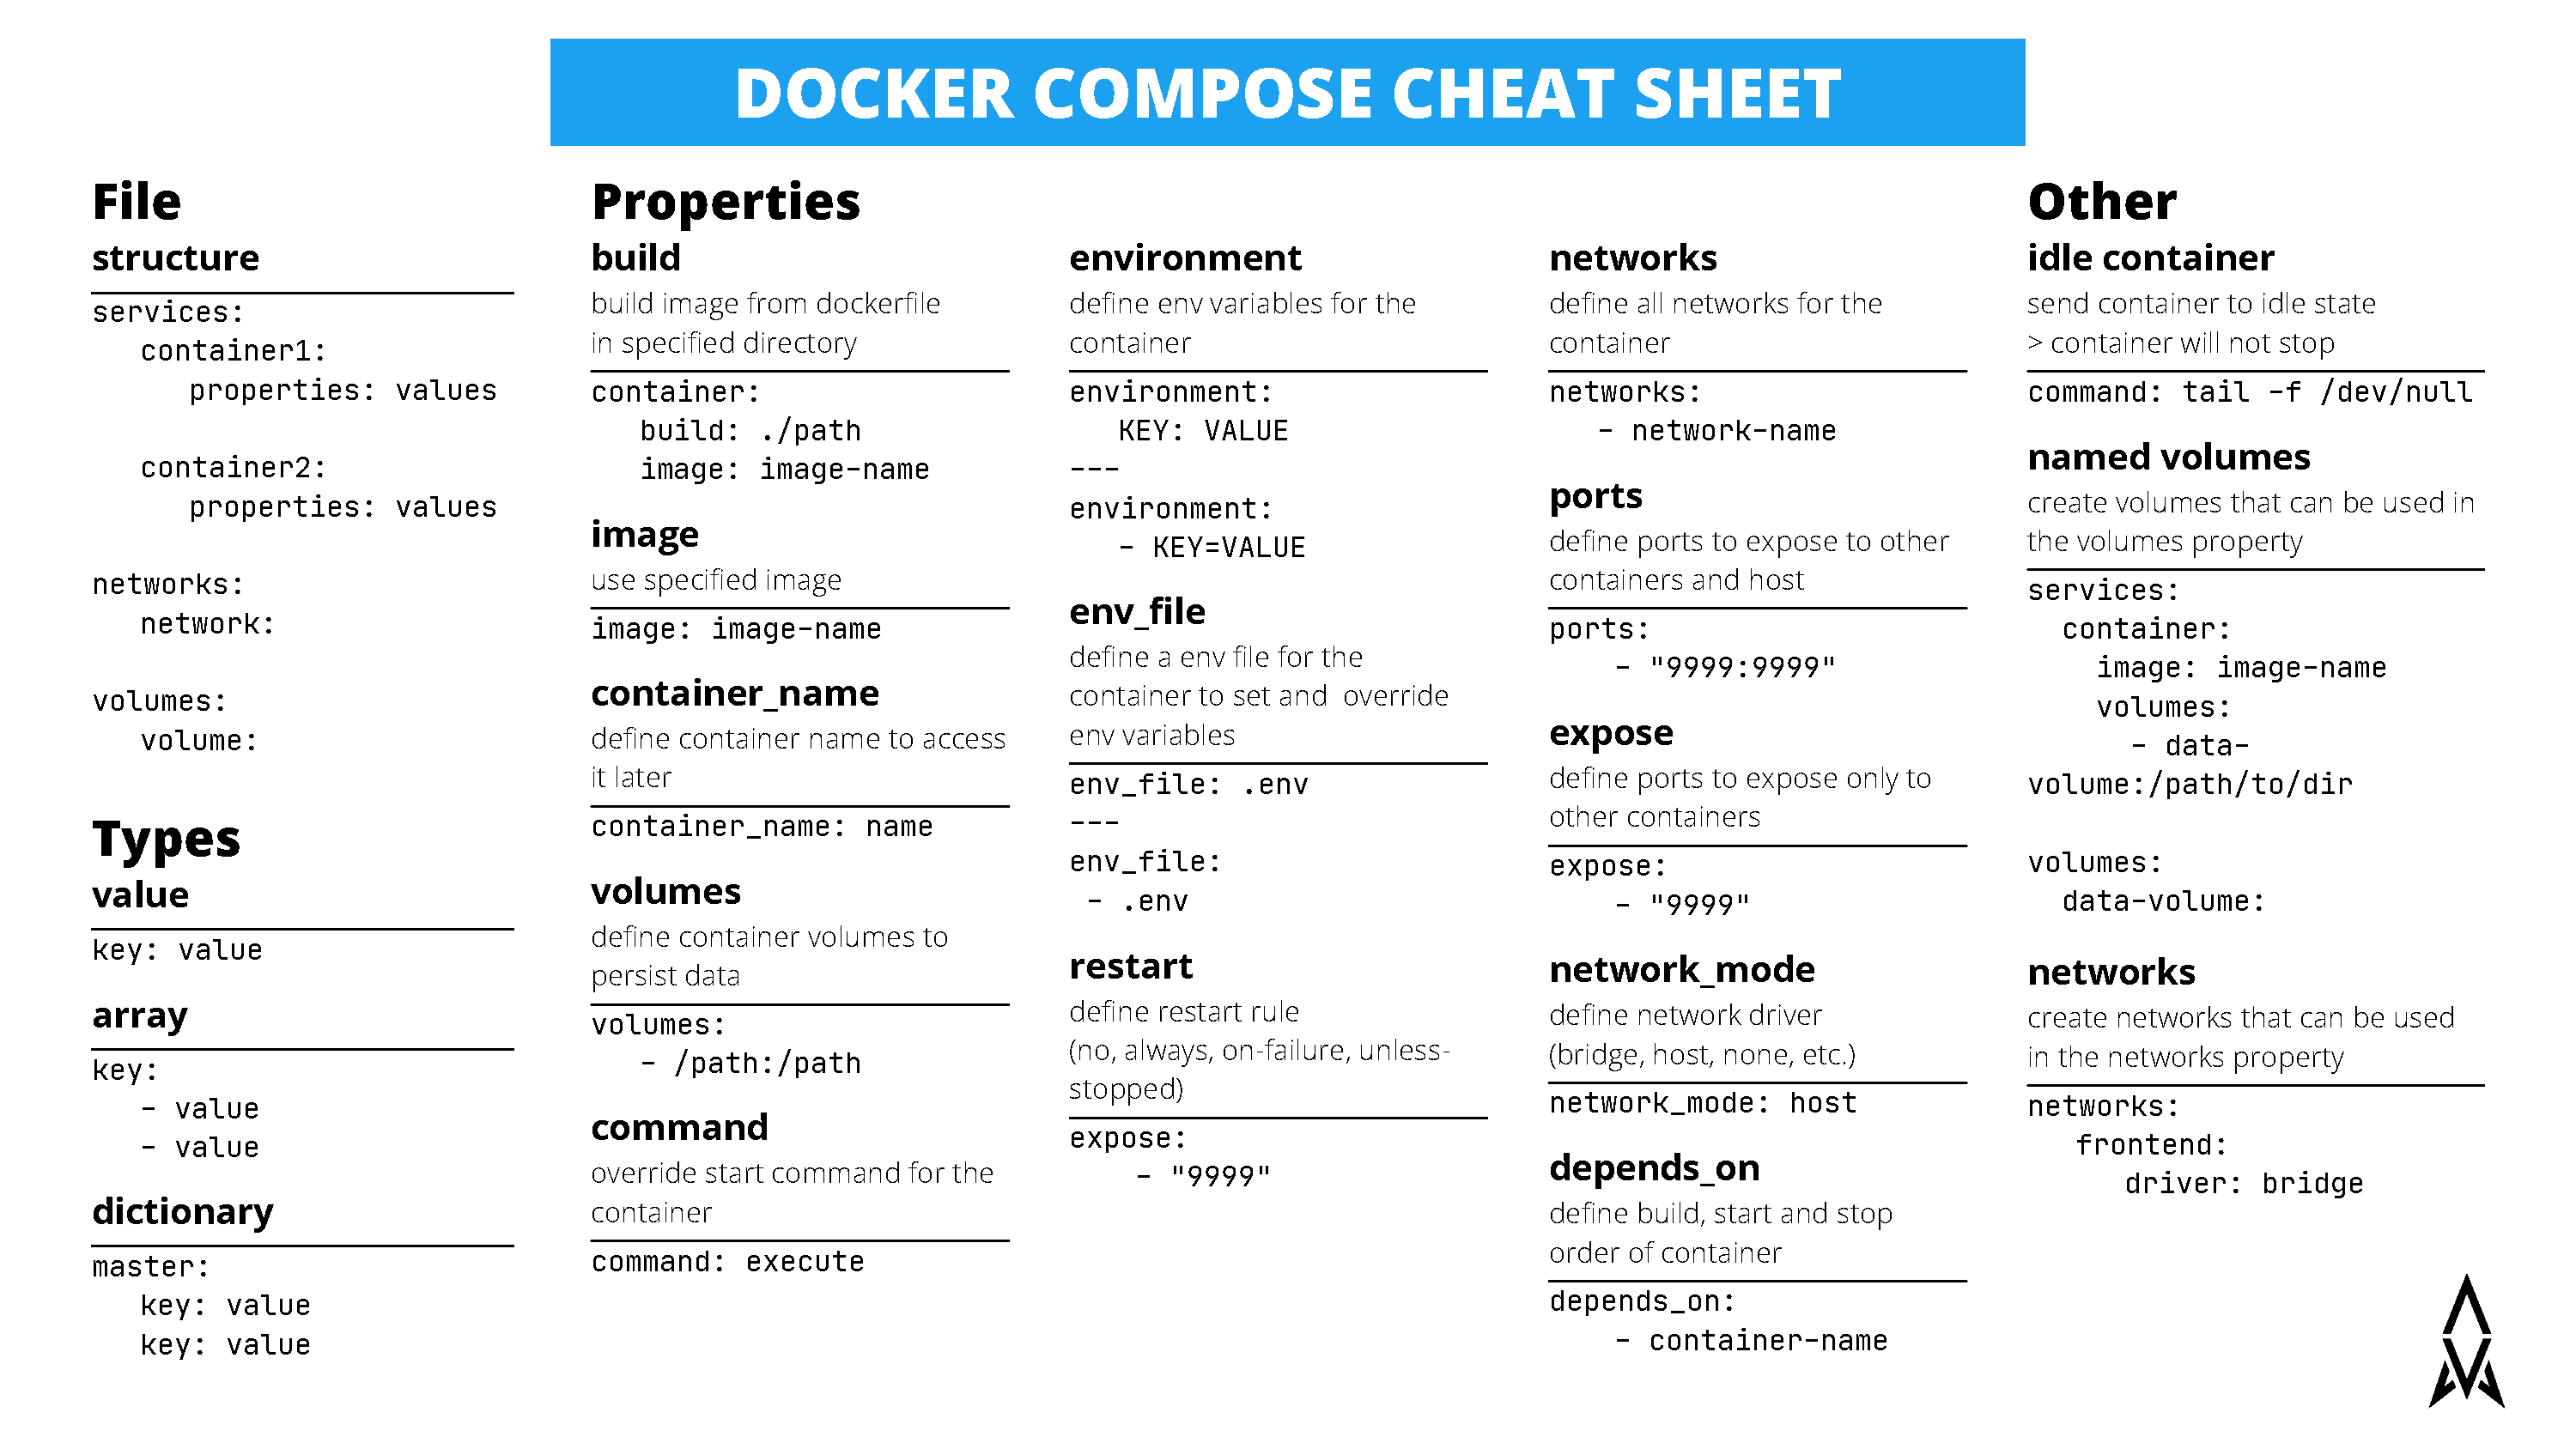
\includegraphics[width=0.9\textwidth]{images/docker-compose-cheat-sheet.pdf}
\end{frame}

\subsection{Singularity}
\begin{frame}[<+->]{Singularity history}
\begin{itemize}
\item Also a container manager as Docker
\item Open-source project
\item Release in 2015
\item Fork project in 2020 with now AppTainer (linux foundation) and SingularityCE
\item HPC compatible, no root write, integrate ressource managers (slurm)
\item Could use Docker images
\end{itemize}
\only<1>{\centering
\includegraphics[width=0.2\textwidth]{images/singularity_logo.pdf}}
\end{frame}

\begin{frame}[<+->][fragile]{Singularity commands}
\begin{block}{classical commands}
\begin{verbatim}
$ singularity search [image_name]
$ singularity pull [image_name]
$ singularity run [image_name]
\end{verbatim}
\end{block}
\end{frame}

\begin{frame}[<+->][fragile]{Singularity and Docker}
\begin{block}{Singularity can use Docker images}
\begin{verbatim}
$ singularity pull docker://debian:latest
INFO:    Converting OCI blobs to SIF format
INFO:    Starting build...
Getting image source signatures
Copying blob f606d8928ed3 done  
Copying config 0311b76201 done  
Writing manifest to image destination
Storing signatures
2022/10/06 10:50:41  info unpack layer: sha256:f606d8928ed378229f2460b94b504cca239fb906efc57acbdf9340bd298d5ddf
INFO:    Creating SIF file...
\end{verbatim}
\end{block}
\end{frame}
